%definira klasu dokumenta 
\documentclass[12pt]{report} 

%prostor izmedu naredbi \documentclass i \begin{document} se zove uvod. U njemu se nalaze naredbe koje se odnose na cijeli dokument

%osnovni LaTex ne može riješiti sve probleme, pa se koriste različiti paketi koji olakšavaju izradu željenog dokumenta
\usepackage[croatian]{babel} 
\usepackage{amssymb}
\usepackage{amsmath}
\usepackage{txfonts}
\usepackage{mathdots}
\usepackage{titlesec}
\usepackage{array}
\usepackage{lastpage}
\usepackage{etoolbox}
\usepackage{tabularray}
\usepackage{color, colortbl}
\usepackage{adjustbox}
\usepackage{geometry}
\usepackage[classicReIm]{kpfonts}
\usepackage{hyperref}
\usepackage{fancyhdr}

\usepackage{float}
\usepackage{setspace}
\restylefloat{table}

\usepackage{listings}

\definecolor{dkgreen}{rgb}{0,0.6,0}
\definecolor{gray}{rgb}{0.5,0.5,0.5}
\definecolor{mauve}{rgb}{0.58,0,0.82}

\lstset{frame=tb,
	language=Java,
	aboveskip=3mm,
	belowskip=3mm,
	showstringspaces=false,
	columns=flexible,
	basicstyle={\small\ttfamily},
	numbers=none,
	numberstyle=\tiny\color{gray},
	keywordstyle=\color{blue},
	commentstyle=\color{dkgreen},
	stringstyle=\color{mauve},
	breaklines=true,
	breakatwhitespace=true,
	xleftmargin=0in,
	xrightmargin=0in,
	tabsize=3
}

\patchcmd{\chapter}{\thispagestyle{plain}}{\thispagestyle{fancy}}{}{} %redefiniranje stila stranice u paketu fancyhdr

%oblik naslova poglavlja
\titleformat{\chapter}{\normalfont\huge\bfseries}{\thechapter.}{20pt}{\Huge}
\titlespacing{\chapter}{0pt}{0pt}{40pt}


\linespread{1.3} %razmak između redaka

\geometry{a4paper, left=1in, top=1in,}  %oblik stranice

\hypersetup{ colorlinks, citecolor=black, filecolor=black, linkcolor=black,	urlcolor=black }   %izgled poveznice


%prored smanjen između redaka u nabrajanjima i popisima
\newenvironment{packed_enum}{
	\begin{enumerate}
		\setlength{\itemsep}{0pt}
		\setlength{\parskip}{0pt}
		\setlength{\parsep}{0pt}
	}{\end{enumerate}}

\newenvironment{packed_item}{
	\begin{itemize}
		\setlength{\itemsep}{0pt}
		\setlength{\parskip}{0pt}
		\setlength{\parsep}{0pt}
	}{\end{itemize}}




%boja za privatni i udaljeni kljuc u tablicama
\definecolor{LightBlue}{rgb}{0.9,0.9,1}
\definecolor{LightGreen}{rgb}{0.9,1,0.9}

%Promjena teksta za dugačke tablice
\DefTblrTemplate{contfoot-text}{normal}{Nastavljeno na idućoj stranici}
\SetTblrTemplate{contfoot-text}{normal}
\DefTblrTemplate{conthead-text}{normal}{(Nastavljeno)}
\SetTblrTemplate{conthead-text}{normal}
\DefTblrTemplate{middlehead,lasthead}{normal}{Nastavljeno od prethodne stranice}
\SetTblrTemplate{middlehead,lasthead}{normal}

%podesavanje zaglavlja i podnožja

\pagestyle{fancy}
\lhead{Programsko inženjerstvo}
\rhead{Halo112}
\lfoot{Hakeri}
\cfoot{stranica \thepage/\pageref{LastPage}}
\rfoot{\today}
\renewcommand{\headrulewidth}{0.2pt}
\renewcommand{\footrulewidth}{0.2pt}


\begin{document} 
	
	
	
	\begin{titlepage}
		\begin{center}
			\vspace*{\stretch{1.0}} %u kombinaciji s ostalim \vspace naredbama definira razmak između redaka teksta
			\LARGE Programsko inženjerstvo\\
			\large Ak. god. 2021./2022.\\
			
			\vspace*{\stretch{3.0}}
			
			\huge Halo112\\
			\Large Dokumentacija, Rev. \textit{2}\\
			
			\vspace*{\stretch{12.0}}
			\normalsize
			Grupa: \textit{$Hakeri$}\\
			Voditelj: \textit{Luka Ivanković}\\
			
			
			\vspace*{\stretch{1.0}}
			Datum predaje: \textit{14. 01. 2022.}\\
	
			\vspace*{\stretch{4.0}}
			
			Nastavnik: \textit{Hrvoje Nuić}\\
		
		\end{center}

	
	\end{titlepage}

	
	\tableofcontents


	\chapter{Dnevnik promjena dokumentacije}
		
		\textbf{\textit{Kontinuirano osvježavanje}}\\
				
		
		\begin{longtblr}[
				label=none
			]{
				width = \textwidth, 
				colspec={|X[2]|X[13]|X[3]|X[3]|}, 
				rowhead = 1
			}
			\hline
			\textbf{Rev.}	& \textbf{Opis promjene/dodatka} & \textbf{Autori} & \textbf{Datum}\\[3pt] \hline
			0.1 & Napravljen predložak.	& Luka Ivanković & 26.10.2021. 		\\[3pt] \hline 
			0.2	& Napisan dio obrazaca upotrebe & Krunoslav Zadrić & 27.10.2021. 	\\[3pt] \hline 
			0.3.1 & Napisani svi obrasci uporabe. & Florijan Rusac & 28.10.2021. \\[3pt] \hline 
			0.3.2	& Dorada obrazaca upotrebe & Krunoslav Zadrić & 29.10.2021. 	\\[3pt] \hline 
			0.3.3 & Dijagram obrazaca uporabe & Leon Banko, Lukas Ujčić & 29.10.2021. \\[3pt] \hline 
			0.3.4 & Sekvencijski dijagrami & Leon Banko, Lukas Ujčić & 30.10.2021. \\[3pt] \hline 
			0.6 & Opis projektnog zadatka & Luka Ivanković & 7.11.2021. \\[3pt] \hline 
			0.7 & Arhitektura baze podataka & Krunoslav Zadrić & 9.11.2021. 	\\[3pt] \hline 
			0.7.1 & Započeli dijagrame razreda & Leon Banko, Lukas Ujčić & 9.11.2021. \\[3pt] \hline 
			0.8 & Povijest rada i trenutni status implementacije,\newline Zaključci i plan daljnjeg rada & * & 28.08.2013. \\[3pt] \hline 
			0.9 & Opisi obrazaca uporabe & * & 07.09.2013. \\[3pt] \hline 
			0.10 & Preveden uvod & * & 08.09.2013. \\[3pt] \hline 
			0.12.2 & Nastavak dijagrama razreda & * & 11.09.2013. \\[3pt] \hline 
			\textbf{1.0} & Verzija samo s bitnim dijelovima za 1. ciklus & * & 11.09.2013. \\[3pt] \hline 
			1.1 & Uređivanje teksta -- funkcionalni i nefunkcionalni zahtjevi & * \newline * & 14.09.2013. \\[3pt] \hline 
			1.2 & Manje izmjene:Timer - Brojilo vremena & * & 15.09.2013. \\[3pt] \hline 
			1.3 & Popravljeni dijagrami obrazaca uporabe & * & 15.09.2013. \\[3pt] \hline 
			1.5 & Generalna revizija strukture dokumenta & * & 19.09.2013. \\[3pt] \hline 
			1.5.1 & Manja revizija (dijagram razmještaja) & * & 20.09.2013. \\[3pt] \hline 
			\textbf{2.0} & Konačni tekst predloška dokumentacije  & * & 28.09.2013. \\[3pt] \hline 
			&  &  & \\[3pt] \hline	
		\end{longtblr}
	
	
		\textit{Moraju postojati glavne revizije dokumenata 1.0 i 2.0 na kraju prvog i drugog ciklusa. Između tih revizija mogu postojati manje revizije već prema tome kako se dokument bude nadopunjavao. Očekuje se da nakon svake značajnije promjene (dodatka, izmjene, uklanjanja dijelova teksta i popratnih grafičkih sadržaja) dokumenta se to zabilježi kao revizija. Npr., revizije unutar prvog ciklusa će imati oznake 0.1, 0.2, …, 0.9, 0.10, 0.11.. sve do konačne revizije prvog ciklusa 1.0. U drugom ciklusu se nastavlja s revizijama 1.1, 1.2, itd.}
	\chapter{Opis projektnog zadatka}
		
		\text Cilj ovog projekta je razviti programsku podršku za stvaranje web aplikacije „Halo112“. To je aplikacija za olakšavanje koordinacije između rada svih spasilačkih službi. Neregistriranom korisniku se pojavljuje stranica za prijavu. Potrebno je unijeti korisničko ime i lozinku. Ispod polja za unos postoji hiperlink „registriraj se“ – vodi korisnika na stranicu za registraciju.
		 
		\text Na stranici za registraciju potrebno je unijeti osobne podatke:
		
		\begin{packed_item}
			\item \text korisničko ime
			\item \text lozinka (potrebno je dva puta upisati lozinku na dva različita polja za tekst radi sigurnosti)
			\item \text ime
			\item \text prezime 
			\item \text email adresa
			\item \text broj mobitela
			\item \text fotografija(opcionalno)
		\end{packed_item}
		\text Sve osim podataka na kojima piše opcionalno su obavezni za unos, i ne može se nastaviti ako nisu popunjena. Osim osobnih podataka, treba se odabrati i uloga:
		
		\begin{packed_item}
			\item \text dispečer 
			\item \text doktor
			\item \text vatrogasac
			\item \text policajac
		\end{packed_item}
		
		\textbf{\text{Korisnik}}\\
		\text Nakon što je korisnik popunio sva potrebna polja, na dnu stranice postoji gumb „pošalji prijavnicu“. Ako se prelazi mišem preko gumba može se vidjeti: „Administrator mora odobriti vašu prijavu“. Klikom na gumb dešavaju se dvije stvari: administratoru dolazi obavijest o registraciji novog korisnika (on može odobriti ili onemogućiti prijavu i također vidi popis svih ostalih registriranih korisnika), korisnika se šalje na novu stranicu. Na stranici piše: „Obavijestit ćemo vas e-mailom kada administrator odobri vašu prijavnicu.“. Ispod natpisa postoji hiperlink „vrati se na stranicu za prijavu“.
		
		\textbf{\text{Administrator}}\\
		\text Administratoru se nakon prijave u sustav prikazuje, na početnoj stranici, popis korisnika kojima se čeka potvrda registracije. On može odobriti registraciju ili odbiti, čime će se automatski poslati mail korisniku o odobrenju/otkazanju njegove registracije. Na posebnoj stranici ima popis korisnika u sustavu. Svakom korisniku ima pristup u osobne podatke i podatke o ulozi (dispečer, doktor, vatrogasac ili policajac). Sve od navedenog administrator može promijeniti. Na trećoj stranici postoji popis stanica u gradu koje može dodavati ili brisati.
		
		\textbf{\text{Spasioci}}\\
		\text Doktori, vatrogasci i policajci su spasioci. Svaki spasilac pripada nekoj stanici (npr. KBC Rebro, PP Trešnjevka, VP Dubrava.) Kojoj stanici pripada određuje voditelj te stanice (on je isto spasilac). Spasilac će trebati raditi određene akcije spašavanja, i ponekad neće biti dostupan (izvan radnog vremena, trenutno izvodi drugu akciju). On može ručno namjestit da li je spreman ili nije u postavkama profila, a dok izvodi drugu akciju automatski se postavlja da je nespreman za ostale akcije.\\
		Ako spasilac ne izvodi trenutno nikakvu akciju i ako je slobodan prikazuje mu se tablica sa zahtjevima za uključivanje u akcije (Akcije zadaje dispečer u posebnom sučelju). On se može odazvati na jednu od ponuđenih akcija (ako ih uopće ima). Za svaku akciju postoje detalji. Prikazuju se neke opće informacije o opisu problema, kolika je razina hitnosti za obradu akcije i kako bi se spasilac kojemu je zahtjev poslan trebao odazvati (pješke, autom, motorom...). Mogu se prikazati i fotografije. Nakon što se odazvao na neku akciju, ne može odabrati drugu dok ova akcija nije završena ili dok ga dispečer nije uklonio s trenutne akcije.\\
		Spasiteljima koji su aktivni na nekoj akciji na početnoj im se stranici ne prikazuje više tablica ponuđenih akcija, nego mapa grada. Na mapi grada nalazi se sve vezano uz trenutnu akciju, može vidjeti sve ostale spasioce koji trenutno sudjeluju u toj akciji i na karti mu se prikazuju zadaci koje može izvoditi. Svaki zadatak je statičan i prikazuje se na mapi kao točka. Ako se mišem stisne na zadatak mogu se vidjeti detalji zadatka. U detaljima piše kratki komentar što se treba obaviti i kako. Za neke zadatke može se na mapi prikazati ruta, kao put kojim bi spasilac trebao doći do lokacije.
		
	
		\textbf{\text{Voditelj Stanice}}\\
		\text Voditelj stanice ponaša se isto kao običan spasilac u gotovo svemu. Specijalno kod njega je što ima posebnu stranicu gdje može odabrati koji spasioci su dio njegove stanice. Također definira na koji su način spasilaci osposobljeni voditi spašavanje. Doktor može biti osposobljen za vožnju motociklom ili kao putnik u kolima hitne pomoći. Vatrogasac može biti osposobljen za vožnju autocisterni, autoljestvi, zapovjednog vozila i šumskog vozila. Policajac se može kretati pješke kao kontaktni policajac, pomoću motocikla, automobila i oklopnog vozila.
		
		\textbf{\text{Dispečer}}\\
		\text Dispečer na temelju prijave otvara akcije spašavanja s dostupnim informacijama i fotografijama. Dispečer vidi broj dostupnih spasioca po stanicama i može poslati zahtjev za uključivanjem spasilaca u akciju spašavanja. Prilikom slanja zahtjeva dispečer definira na koji način bi spasilac trebao sudjelovati (auto, pješke.. ) i koja je razina hitnosti. Spasioci koji zadovoljavaju kriterije se mogu odazvati na akciju. Dispečer, ako je to potrebno, može spasioca ukloniti s akcije. Ako je akcija spašavanja završila, dispečer je u sustavu može označiti kao gotovom.\\
		Dispečer preko karte spasiocima pojedinačno zadaje zadatke. Zadatak može tražiti prolazak određenom rutom i dolazak do određene lokacije. Svaki zadatak može imati i dodatan komentar od dispečera. Za izračun ruta koje prate staze i ceste koristi se vanjski servis OSRM2. \\
		Dispečeru se na temelju trenutnih pozicija spasilaca prikazuje Voronojev dijagram. Dispečer može odabrati da se za izradu dijagrama koriste pozicije svih spasioca, ili svih dostupnih neaktivnih spasioca, ili aktivnih spasioca na određenoj akciji. Ovisno o načinu na koji spasilac sudjeluje u akciji, dispečeru se na karti prikazuje drugačija ikona.
		
	
		\textbf{\text{Potencijalna korist projekta}}\\
		\text Ovaj projekt mogao bi biti od velike koristi bilo kojoj spasilačkoj službi jer jako olakšava komunikaciju između služba. Ako se dogodi nekakva nesreća/problem, puno prije i lakše spasioci mogu iskomunicirati tko se i gdje treba nalaziti da što prije otklone problem.
		
		\textbf{\text{Postojeća slična rješenja}}\\
		\text Slično rješenje u svijetu je belgijska aplikacija "112 BE". "112 BE" je besplatna službena aplikacija belgijskog tima za hitne slučajeve (policija, vatrogasci, hitna pomoć). Nakon registracije u aplikaciju moguće je komentirati službu za korisnike koja uz pomoć vaše lokacije odabire najbliže spasioce koje treba poslati. U ovoj verziji se komunicira preko  interneta no ukoliko nema interneta postoji i mogućnost SMS poruka koja je u ovom slučaju besplatna. Također ukoliko osoba nije u mogućnosti govoriti otvara se chat kako bi se moglo komunicirati  


		\begin{figure}[H]
			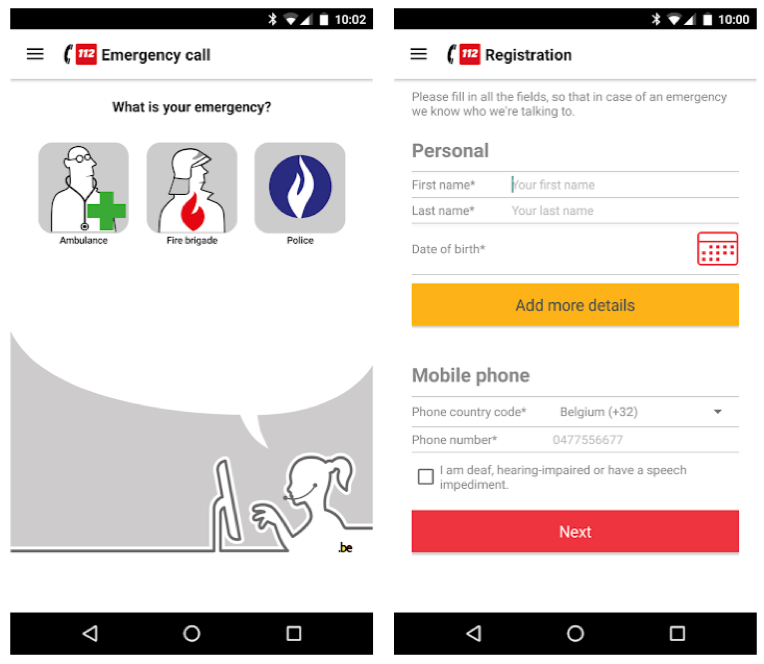
\includegraphics[scale=0.5]{slike/112-app-options.PNG}
			\centering
			\caption{Primjer postojećeg rješenja}
			\label{fig:112_BE}
			\end{figure}
		
		\textbf{\text{Skup korisnika koji bi mogao biti zainteresiran za ostvareno rješenje}}\\
		\text Ovaj projekt može koristiti bilo kakav spasilac. Vrlo vjerojatno bi voditelj stanice određivao bi li se koristila aplikacija ili ne. Ako se odluči da bi aplikacija bila korisna mogao bi ju uvesti kao obavezno sredstvo za komuniciranje između svojih spasilaca. Organizacija bi im se odmah poboljšala.
		
		\textbf{\text{Mogućnost prilagodbe rješenja}}\\
		\text Ovaj program je jako fleksibilan i može se uvesti jako puno različitih funkcionalnosti. Ako se tijekom izrade programa neka funkcionalnost čini redundantna, može se lako zamjeniti drugom ili ukloniti. Dodatne funkcionalnosti se također vrlo lako mogu dodavati.
		
		\textbf{\text{Opseg projektnog zadatka}}\\
		\text Ovaj zadatak se može implementirati na bezbroj različitih načina od kojih postoje i teži i lakši načini. Naravno cilj je napraviti ispravan i koristiv program, a ne si olakšavati ili otežavati zadatak radi posla. Svaku funkcionalnost potrebno je dodati na prvenstveno ispravan način bez nepotrebnog otežavanja zadatka.
		
		\textbf{\text{Moguće nadogradnje projektnog zadatka}}\\
		\text Ovaj zadatak se može vrlo jednostavno urediti naknadno. Uz ideju nekog voditelja stanice mogle bi se dodati nove funkcionalnosti za tu stanicu ili za sve korisnike.
		
		
		\eject
		
		
		
	
	\chapter{Specifikacija programske potpore}
		
	\section{Funkcionalni zahtjevi}
			
			\textbf{\textit{dio 1. revizije}}\\
			
			\textit{Navesti \textbf{dionike} koji imaju \textbf{interes u ovom sustavu} ili  \textbf{su nositelji odgovornosti}. To su prije svega korisnici, ali i administratori sustava, naručitelji, razvojni tim.}\\
				
			\textit{Navesti \textbf{aktore} koji izravno \textbf{koriste} ili \textbf{komuniciraju sa sustavom}. Oni mogu imati inicijatorsku ulogu, tj. započinju određene procese u sustavu ili samo sudioničku ulogu, tj. obavljaju određeni posao. Za svakog aktora navesti funkcionalne zahtjeve koji se na njega odnose.}\\
			
			
			\noindent \textbf{Dionici:}
			
			\begin{packed_enum}
				
				\item Dionik 1
				\item Dionik 2				
				\item ...
				
			\end{packed_enum}
			
			\noindent \textbf{Aktori i njihovi funkcionalni zahtjevi:}
			
			
			\begin{packed_enum}
				
				
				\begin{packed_enum}

					\item funkcionalnost 1\item  \underbar{Aktor 1 (inicijator) može:}
					\item funkcionalnost 2
					\begin{packed_enum}
						
						\item  podfunkcionalnost 1 
						\item  podfunkcionalnost 2
				
					\end{packed_enum}
					\item  funkcionalnost 3
					
				\end{packed_enum}
			
				\item  \underbar{Aktor 2 (sudionik) može:}
				
				\begin{packed_enum}
					
					\item funkcionalnost 1
					\item funkcionalnost 2
					
				\end{packed_enum}
			\end{packed_enum}
			
			\eject 
			
			
				
			\subsection{Obrasci uporabe}
				
				\textbf{\textit{dio 1. revizije}}
				
				\subsubsection{Opis obrazaca uporabe}
					\textit{Funkcionalne zahtjeve razraditi u obliku obrazaca uporabe. Svaki obrazac je potrebno razraditi prema donjem predlošku. Ukoliko u nekom koraku može doći do odstupanja, potrebno je to odstupanje opisati i po mogućnosti ponuditi rješenje kojim bi se tijek obrasca vratio na osnovni tijek.}\\
					

					\noindent \underbar{\textbf{UC$<$broj obrasca$>$ -$<$ime obrasca$>$}}
					\begin{packed_item}
	
						\item \textbf{Glavni sudionik: }$<$sudionik$>$
						\item  \textbf{Cilj:} $<$cilj$>$
						\item  \textbf{Sudionici:} $<$sudionici$>$
						\item  \textbf{Preduvjet:} $<$preduvjet$>$
						\item  \textbf{Opis osnovnog tijeka:}
						
						\item[] \begin{packed_enum}
	
							\item $<$opis korak jedan$>$
							\item $<$opis korak dva$>$
							\item $<$opis korak tri$>$
							\item $<$opis korak četiri$>$
							\item $<$opis korak pet$>$
						\end{packed_enum}
						
						\item  \textbf{Opis mogućih odstupanja:}
						
						\item[] \begin{packed_item}
	
							\item[2.a] $<$opis mogućeg scenarija odstupanja u koraku 2$>$
							\item[] \begin{packed_enum}
								
								\item $<$opis rješenja mogućeg scenarija korak 1$>$
								\item $<$opis rješenja mogućeg scenarija korak 2$>$
								
							\end{packed_enum}
							\item[2.b] $<$opis mogućeg scenarija odstupanja u koraku 2$>$
							\item[3.a] $<$opis mogućeg scenarija odstupanja  u koraku 3$>$
							
						\end{packed_item}
					\end{packed_item}

					\noindent \underbar{\textbf{UC$<$broj obrasca$>$ - \text Osvježavanje dostupnosti}}
					\begin{packed_item}
	
						\item \textbf{Glavni sudionik: }\text Spasilac
						\item  \textbf{Cilj:} \text Ažurirati dostupnost za akciju
						\item  \textbf{Sudionici:} \text Baza podataka
						\item  \textbf{Preduvjet:} \text Spasilac prijavljen
						\item  \textbf{Opis osnovnog tijeka:}
						
						\item[] \begin{packed_enum}
	
							\item Spasilac klikom na gumb odabire svoju dostupnost
							\item Spasilac postaje dostupan ili nedostupan za akciju
						\end{packed_enum}
					\end{packed_item}

					\noindent \underbar{\textbf{UC$<$broj obrasca$>$ - \text Definiranje spasilaca }}
					\begin{packed_item}
	
						\item \textbf{Glavni sudionik: }\text Voditelj
						\item  \textbf{Cilj:} \text Definirati spasioce i njihove uloge
						\item  \textbf{Sudionici:} \text Baza podataka
						\item  \textbf{Preduvjet:} \text Voditelj prijavljen
						\item  \textbf{Opis osnovnog tijeka:}
						
						\item[] \begin{packed_enum}
	
							\item \text Voditelj odabire opciju pregleda stanice
							\item \text Voditelj dobiva pregled stanice, opreme u stanici i spasilaca pripadnika stanice
							\item \text Voditelj odabire opciju dodavanja spasilaca
							\item \text Voditelj odabire spasioca iz baze registriranih spasilaca te mu dodjeljuje ulogu
					
						\end{packed_enum}

						\item  \textbf{Opis mogućih odstupanja:}
						
						\item[] \begin{packed_item}
	
							\item[4.a] \text Nema slobodnih spasilaca
							\item[] \begin{packed_item}
								
								\item \text Sustav obavještava voditelja da nema dostupnih spasilaca
								
							\end{packed_item}
							
						\end{packed_item}
						
					\end{packed_item}

					\noindent \underbar{\textbf{UC$<$broj obrasca$>$ - \text Otvaranje akcije}}
					\begin{packed_item}
	
						\item \textbf{Glavni sudionik: }\text Dispečer
						\item  \textbf{Cilj:} \text Otvoriti akciju i poslati zahtjeve spasiocima
						\item  \textbf{Sudionici:} \text Baza podataka
						\item  \textbf{Preduvjet:} \text Dispečer prijavljen
						\item  \textbf{Opis osnovnog tijeka:}
						
						\item[] \begin{packed_enum}
	
							\item \text Dispečer otvara akciju sa dostupnim informacijama i fotografijama
							\item \text Dispečer dobiva uvid u broj spasilaca po stanicama
							\item \text Dispečer šalje zahtjev pojedinom spasiocu sa definiranim načinom sudjelovanja i hitnosti
						\end{packed_enum}
						
						\item  \textbf{Opis mogućih odstupanja:}
						
						\item[] \begin{packed_item}
	
							\item[2.a] \text Nema dostupnih spasilaca za akciju
							\item[] \begin{packed_item}
								
								\item \text Sustav obavještava dispečera o nedostupnosti spasilaca
								
							\end{packed_item}
							
						\end{packed_item}
					\end{packed_item}

					\noindent \underbar{\textbf{UC$<$broj obrasca$>$ - \text Završavanje akcije}}
					\begin{packed_item}
	
						\item \textbf{Glavni sudionik: }\text Dispečer
						\item  \textbf{Cilj:}\text Označiti akciju kao završenom
						\item  \textbf{Sudionici:} Baza podataka
						\item  \textbf{Preduvjet:} Akcija završena
						\item  \textbf{Opis osnovnog tijeka:}
						
						\item[] \begin{packed_enum}
	
							\item \text Dispečer provjerava je li akcija završena
							\item \text Dispečer označava akciju kao završenom
						\end{packed_enum}
						
					\end{packed_item}
				
					
				\subsubsection{Dijagrami obrazaca uporabe}
					
					\textit{Prikazati odnos aktora i obrazaca uporabe odgovarajućim UML dijagramom. Nije nužno nacrtati sve na jednom dijagramu. Modelirati po razinama apstrakcije i skupovima srodnih funkcionalnosti.}
				\eject		
				
			\subsection{Sekvencijski dijagrami}
				
				\textbf{\textit{dio 1. revizije}}\\
				
				\textit{Nacrtati sekvencijske dijagrame koji modeliraju najvažnije dijelove sustava (max. 4 dijagrama). Ukoliko postoji nedoumica oko odabira, razjasniti s asistentom. Uz svaki dijagram napisati detaljni opis dijagrama.}
				\eject
	
		\section{Ostali zahtjevi}
		
			\textbf{\textit{dio 1. revizije}}\\
		 
			 \textit{Nefunkcionalni zahtjevi i zahtjevi domene primjene dopunjuju funkcionalne zahtjeve. Oni opisuju \textbf{kako se sustav treba ponašati} i koja \textbf{ograničenja} treba poštivati (performanse, korisničko iskustvo, pouzdanost, standardi kvalitete, sigurnost...). Primjeri takvih zahtjeva u Vašem projektu mogu biti: podržani jezici korisničkog sučelja, vrijeme odziva, najveći mogući podržani broj korisnika, podržane web/mobilne platforme, razina zaštite (protokoli komunikacije, kriptiranje...)... Svaki takav zahtjev potrebno je navesti u jednoj ili dvije rečenice.}
			 
			 
			 
	
	\chapter{Arhitektura i dizajn sustava}
		
		\textbf{\textit{dio 1. revizije}}\\

		\textit{ Potrebno je opisati stil arhitekture te identificirati: podsustave, preslikavanje na radnu platformu, spremišta podataka, mrežne protokole, globalni upravljački tok i sklopovsko-programske zahtjeve. Po točkama razraditi i popratiti odgovarajućim skicama:}
	\begin{itemize}
		\item 	\textit{izbor arhitekture temeljem principa oblikovanja pokazanih na predavanjima (objasniti zašto ste baš odabrali takvu arhitekturu)}
		\item 	\textit{organizaciju sustava s najviše razine apstrakcije (npr. klijent-poslužitelj, baza podataka, datotečni sustav, grafičko sučelje)}
		\item 	\textit{organizaciju aplikacije (npr. slojevi frontend i backend, MVC arhitektura) }		
	\end{itemize}

	
		

		

				
		\section{Baza podataka}
			
			\textbf{\textit{dio 1. revizije}}\\
			
		\textit{Potrebno je opisati koju vrstu i implementaciju baze podataka ste odabrali, glavne komponente od kojih se sastoji i slično.}
		
			\subsection{Opis tablica}
			

				\textit{Svaku tablicu je potrebno opisati po zadanom predlošku. Lijevo se nalazi točno ime varijable u bazi podataka, u sredini se nalazi tip podataka, a desno se nalazi opis varijable. Svjetlozelenom bojom označite primarni ključ. Svjetlo plavom označite strani ključ}
				
				
				\begin{longtblr}[
					label=none,
					entry=none
					]{
						width = \textwidth,
						colspec={|X[6,l]|X[6, l]|X[20, l]|}, 
						rowhead = 1,
					} %definicija širine tablice, širine stupaca, poravnanje i broja redaka naslova tablice
					\hline \multicolumn{3}{|c|}{\textbf{korisnik - ime tablice}}	 \\ \hline[3pt]
					\SetCell{LightGreen}IDKorisnik & INT	&  	Lorem ipsum dolor sit amet, consectetur adipiscing elit, sed do eiusmod  	\\ \hline
					korisnickoIme	& VARCHAR &   	\\ \hline 
					email & VARCHAR &   \\ \hline 
					ime & VARCHAR	&  		\\ \hline 
					\SetCell{LightBlue} primjer	& VARCHAR &   	\\ \hline 
				\end{longtblr}
				
				
			
			\subsection{Dijagram baze podataka}
				\textit{ U ovom potpoglavlju potrebno je umetnuti dijagram baze podataka. Primarni i strani ključevi moraju biti označeni, a tablice povezane. Bazu podataka je potrebno normalizirati. Podsjetite se kolegija "Baze podataka".}
			
			\eject
			
			
		\section{Dijagram razreda}
		
			\textit{Potrebno je priložiti dijagram razreda s pripadajućim opisom. Zbog preglednosti je moguće dijagram razlomiti na više njih, ali moraju biti grupirani prema sličnim razinama apstrakcije i srodnim funkcionalnostima.}\\
			
			\textbf{\textit{dio 1. revizije}}\\
			
			\textit{Prilikom prve predaje projekta, potrebno je priložiti potpuno razrađen dijagram razreda vezan uz \textbf{generičku funkcionalnost} sustava. Ostale funkcionalnosti trebaju biti idejno razrađene u dijagramu sa sljedećim komponentama: nazivi razreda, nazivi metoda i vrste pristupa metodama (npr. javni, zaštićeni), nazivi atributa razreda, veze i odnosi između razreda.}\\
			
			\textbf{\textit{dio 2. revizije}}\\			
			
			\textit{Prilikom druge predaje projekta dijagram razreda i opisi moraju odgovarati stvarnom stanju implementacije}
			
			
			
			\eject
		
		\section{Dijagram stanja}
			
			
			\textbf{\textit{dio 2. revizije}}\\
			
			\textit{Potrebno je priložiti dijagram stanja i opisati ga. Dovoljan je jedan dijagram stanja koji prikazuje \textbf{značajan dio funkcionalnosti} sustava. Na primjer, stanja korisničkog sučelja i tijek korištenja neke ključne funkcionalnosti jesu značajan dio sustava, a registracija i prijava nisu. }
			
			
			\eject 
		
		\section{Dijagram aktivnosti}
			
			\textbf{\textit{dio 2. revizije}}\\
			
			 \textit{Potrebno je priložiti dijagram aktivnosti s pripadajućim opisom. Dijagram aktivnosti treba prikazivati značajan dio sustava.}
			
			\eject
		\section{Dijagram komponenti}
		
			\textbf{\textit{dio 2. revizije}}\\
		
			 \textit{Potrebno je priložiti dijagram komponenti s pripadajućim opisom. Dijagram komponenti treba prikazivati strukturu cijele aplikacije.}
	\chapter{Implementacija i korisničko sučelje}
		
		
		\section{Korištene tehnologije i alati}
			 
			 \noindent \underbar{\textbf{MiKTeX}}
			 \begin{packed_item}
			 	\item  \textbf{Opis:} MiKTeX je besplatna distribucija otvorenog koda TeX/LaTeX sustava za Microsoft Windows.
			 	\item  \textbf{Mjesto primjene:} Projektna dokumentacija
			 	\item  \textbf{Poveznica:} https://miktex.org/
			 \end{packed_item}
		
			\noindent \underbar{\textbf{Visual paradigm}}
			\begin{packed_item}
				\item  \textbf{Opis:} Visual paradigm je UML CASE alat koji se koristi za stvaranje UML dijagrama.
				\item  \textbf{Mjesto primjene:} Projektna dokumentacija
				\item  \textbf{Poveznica:} https://www.visual-paradigm.com/
			\end{packed_item}
		
			\noindent \underbar{\textbf{Java Spring Framework}}
			\begin{packed_item}
				\item  \textbf{Opis:} Java Spring Framework je razvojni okvir otvorenog koda za stvaranje samostalnih aplikacija koje se pokreću na Java Virtual Machine-u (JVM).
				\item  \textbf{Mjesto primjene:} Web aplikacija - backend
				\item  \textbf{Poveznica:} https://spring.io/projects/spring-framework/
			\end{packed_item}
		
			\noindent \underbar{\textbf{React}}
			\begin{packed_item}
				\item  \textbf{Opis:} React je besplatna JavaScript biblioteka otvorenog koda za izgradnju korisničkih sučelja.
				\item  \textbf{Mjesto primjene:} Web aplikacija - frontend
				\item  \textbf{Poveznica:} https://reactjs.org/
			\end{packed_item}
		
			\noindent \underbar{\textbf{Leaflet}}
			\begin{packed_item}
				\item  \textbf{Opis:} Leaflet je JavaScript biblioteka otvorenog koda koja se koristi za izradu web aplikacija s kartama.
				\item  \textbf{Mjesto primjene:} Web aplikacija - frontend
				\item  \textbf{Poveznica:} http://leafletjs.com/
			\end{packed_item}
		
			\noindent \underbar{\textbf{Heroku}}
			\begin{packed_item}
				\item  \textbf{Opis:} Heroku je cloud platforma kao usluga (PaaS) koja podržava nekoliko programskih jezika.
				\item  \textbf{Mjesto primjene:} Puštanje aplikacije u pogon
				\item  \textbf{Poveznica:} https://www.heroku.com/
			\end{packed_item}
			\eject 
		
	
		\section{Ispitivanje programskog rješenja}
			
			\textbf{\textit{dio 2. revizije}}\\
			
			 \textit{U ovom poglavlju je potrebno opisati provedbu ispitivanja implementiranih funkcionalnosti na razini komponenti i na razini cijelog sustava s prikazom odabranih ispitnih slučajeva. Studenti trebaju ispitati temeljnu funkcionalnost i rubne uvjete.}
	
			
			\subsection{Ispitivanje komponenti}
			\textit{Potrebno je provesti ispitivanje jedinica (engl. unit testing) nad razredima koji implementiraju temeljne funkcionalnosti. Razraditi \textbf{minimalno 6 ispitnih slučajeva} u kojima će se ispitati redovni slučajevi, rubni uvjeti te izazivanje pogreške (engl. exception throwing). Poželjno je stvoriti i ispitni slučaj koji koristi funkcionalnosti koje nisu implementirane. Potrebno je priložiti izvorni kôd svih ispitnih slučajeva te prikaz rezultata izvođenja ispita u razvojnom okruženju (prolaz/pad ispita). }
			
			
			
			\subsection{Ispitivanje sustava}
			
			 \textit{Potrebno je provesti i opisati ispitivanje sustava koristeći radni okvir Selenium\footnote{\url{https://www.seleniumhq.org/}}. Razraditi \textbf{minimalno 4 ispitna slučaja} u kojima će se ispitati redovni slučajevi, rubni uvjeti te poziv funkcionalnosti koja nije implementirana/izaziva pogrešku kako bi se vidjelo na koji način sustav reagira kada nešto nije u potpunosti ostvareno. Ispitni slučaj se treba sastojati od ulaza (npr. korisničko ime i lozinka), očekivanog izlaza ili rezultata, koraka ispitivanja i dobivenog izlaza ili rezultata.\\ }
			 
			 \textit{Izradu ispitnih slučajeva pomoću radnog okvira Selenium moguće je provesti pomoću jednog od sljedeća dva alata:}
			 \begin{itemize}
			 	\item \textit{dodatak za preglednik \textbf{Selenium IDE} - snimanje korisnikovih akcija radi automatskog ponavljanja ispita	}
			 	\item \textit{\textbf{Selenium WebDriver} - podrška za pisanje ispita u jezicima Java, C\#, PHP koristeći posebno programsko sučelje.}
			 \end{itemize}
		 	\textit{Detalji o korištenju alata Selenium bit će prikazani na posebnom predavanju tijekom semestra.}
			
			\eject 
		
		
		\section{Dijagram razmještaja}
			
			\textbf{\textit{dio 2. revizije}}
			
			 \textit{Potrebno je umetnuti \textbf{specifikacijski} dijagram razmještaja i opisati ga. Moguće je umjesto specifikacijskog dijagrama razmještaja umetnuti dijagram razmještaja instanci, pod uvjetom da taj dijagram bolje opisuje neki važniji dio sustava.}
			
			\eject 
		
		\section{Upute za puštanje u pogon}
		
			\textbf{\textit{dio 2. revizije}}\\
		
			 \textit{U ovom poglavlju potrebno je dati upute za puštanje u pogon (engl. deployment) ostvarene aplikacije. Na primjer, za web aplikacije, opisati postupak kojim se od izvornog kôda dolazi do potpuno postavljene baze podataka i poslužitelja koji odgovara na upite korisnika. Za mobilnu aplikaciju, postupak kojim se aplikacija izgradi, te postavi na neku od trgovina. Za stolnu (engl. desktop) aplikaciju, postupak kojim se aplikacija instalira na računalo. Ukoliko mobilne i stolne aplikacije komuniciraju s poslužiteljem i/ili bazom podataka, opisati i postupak njihovog postavljanja. Pri izradi uputa preporučuje se \textbf{naglasiti korake instalacije uporabom natuknica} te koristiti što je više moguće \textbf{slike ekrana} (engl. screenshots) kako bi upute bile jasne i jednostavne za slijediti.}
			
			
			 \textit{Dovršenu aplikaciju potrebno je pokrenuti na javno dostupnom poslužitelju. Studentima se preporuča korištenje neke od sljedećih besplatnih usluga: \href{https://aws.amazon.com/}{Amazon AWS}, \href{https://azure.microsoft.com/en-us/}{Microsoft Azure} ili \href{https://www.heroku.com/}{Heroku}. Mobilne aplikacije trebaju biti objavljene na F-Droid, Google Play ili Amazon App trgovini.}
			
			
			\eject 
	\chapter{Zaključak i budući rad}
		

	Sve skupa zadatak je izrađen kvalitetno. Ne savršeno, ima mjesta za popravak ali tim je zadovoljan gotovim rezultatom. Kao tim smo većinom dobro surađivali. Početak projekta (pisanje dokumentacije) tekao je glatko. Prve probleme susreli smo pokušavajući isprogramirati generičke funkcionalnosti, sve je dobro radilo osim ulogiravanja korisnika. CORS greška se tada prvi puta pojavila i sve odtad ju nismo uspjeli rješiti. To je rezultiralo neuspjelim pokušajima deployanja aplikacije na javni poslužitelj (prvo smo isprobali HEROKU). Nekako smo zaobišli problem i uspjeli prijaviti korisnika bez obzira na CORS grešku. Za vrijeme međuispita nismo radili. Zato je bilo teško vratiti se natrag na posao odmah nakon završetka ispita i trebalo je cijelom timu dosta vremena da bi počeli opet kvalitetnije raditi. Oko Božića smo shvatili da nemamo još puno vremena za dovršiti aplikaciju, a da nam je još puno preostalo. No ipak praznici su bili i malo se radilo. Nakon završetka praznika malo pomalo pa je cijeli tim stisnuo i progurao nekako sve funkcionalnosti koje dotad nismo imali. 90 posto aplikacije smo uspjeli napraviti kako treba. \par
	Od funkcionalnosti dugo nam je trebalo da smislimo rješenje za spremanje slika na backend i ta komunikacija (slanje slika sa frontenda na backend i obrnuto). Nakon što smo shvatili da se slika može jednostavno slati kao string unutar JSON-a, trebalo nam je samo koji dan da implementiramo i tu funkconalnost. Velik zalogaj je također bila mapa. Ali nakon što smo uspjeli postaviti mapu da se prikazuje, nije bilo većih problema sa prikazivanjem stvari na mapi. \par
	Nismo našli kvalitetno rješenje za prikazivanje i postavljanje komentara. Teško je bilo postaviti pop-up gdje bi korisnik napisao komentar. Imali smo i problema sa prikazivanjem voronijevih dijagrama, ali smo uspjeli prikazati lokacije korisnika i zadano ih filtrirati (bez dijagrama). \par
	Na backendu nije bilo previše „tehničkih“ poteškoća, više su bile poteškoće organizacije. Pošto je većina rađena u žurbi, nije bilo puno vremena za organizirati adrese za GET i POST. To je rezultiralo teško snalaženje frontend tima i time malo manje kvalitetan rad nego li je mogao biti. Definitivno je bilo puno truda uloženo u cjelokupno programiranje projekta, a time je stečeno i mnogo novih znanja (a i prijateljstava). Na frontendu se najviše naučilo o asinkronosti jezika Javascript i kako pametno manevrirati kroz HTML bez da javascript baci error zbog ne dohvaćanja stavki sa backenda. Na backendu su se naučile osnove rađenja unutar programskog okvira (JavaBeans). Moglo se više toga naučiti o samoj komunikaciji sa frontendom (kako funkcioniraju protokoli i kako dobro organizirati adrese za bolje i sigurnije snalaženje). Mislim da nam je svima nedostajalo znanja o timskom radu u kodiranju, što prvenstveno uključuje uredno i organizirano pisanje kodova (tako da ne može samo autor znati kako bi kod trebao raditi, nego i bilo tko drugi koji čita kod nakon njega). \par
	Kao voditelj tima, također mogu reći da mi je nedostajalo voditeljskog iskustva i da sam puno naučio o vođenju tima. Ima definitivno stvari koje bih učinio drugačije od početka da sam vodim ovaj projekt ispočetka. Na kraju je cijeli tim odlično radio na projektu i prije nastavka bismo definitivno uredili cijeli kod da radi kvalitetnije sad kada razumijemo neke nove stvari. \par

		
		\eject 
	\chapter*{Popis literature}
		\addcontentsline{toc}{chapter}{Popis literature}
	 	
		
		\begin{enumerate}
			
			
			\item  Programsko inženjerstvo, FER ZEMRIS, \url{http://www.fer.hr/predmet/proinz}
			
			\item  I. Sommerville, "Software engineering", 8th ed, Addison Wesley, 2007.
			
			\item  T.C.Lethbridge, R.Langaniere, "Object-Oriented Software Engineering", 2nd ed. McGraw-Hill, 2005.
			
			\item  I. Marsic, Software engineering book``, Department of Electrical and Computer Engineering, Rutgers University, \url{http://www.ece.rutgers.edu/~marsic/books/SE}
			
			\item  The Unified Modeling Language, \url{https://www.uml-diagrams.org/}
			
			\item  Astah Community, \url{http://astah.net/editions/uml-new}
		\end{enumerate}
		
		 
	
	
	\begingroup
	\renewcommand*\listfigurename{Indeks slika i dijagrama}
	%\renewcommand*\listtablename{Indeks tablica}
	%\let\clearpage\relax
	\listoffigures
	%\vspace{10mm}
	%\listoftables
	\endgroup
	\addcontentsline{toc}{chapter}{Indeks slika i dijagrama}


	
	\eject 
		
	\chapter*{Dodatak: Prikaz aktivnosti grupe}
		\addcontentsline{toc}{chapter}{Dodatak: Prikaz aktivnosti grupe}
		
		\section*{Dnevnik sastajanja}
		
		\textbf{\textit{Kontinuirano osvježavanje}}\\
		
		 \textit{U ovom dijelu potrebno je redovito osvježavati dnevnik sastajanja prema predlošku.}
		
		\begin{packed_enum}
			\item  sastanak
			
			\item[] \begin{packed_item}
				\item Datum: 27. listopada 2021.
				\item Prisustvovali: Luka Ivanković, Ante Perković, Lukas Ujčić, Florijan Rusac, Krunoslav Zadrić, Leon Banko
				\item Teme sastanka:
				\begin{packed_item}
					\item  Upoznavanje sa GitLabom
				\end{packed_item}
			\end{packed_item}
			
			\item  sastanak
			\item[] \begin{packed_item}
				\item Datum: 28. listopada 2021.
				\item Prisustvovali: Luka Ivanković, Ante Perković, Lukas Ujčić, Florijan Rusac, Krunoslav Zadrić, Leon Banko, Mario Galić 
				\item Teme sastanka:
				\begin{packed_item}
					\item  Zadavanje zadataka
				\end{packed_item}
			\end{packed_item}

			\item  sastanak
			\item[] \begin{packed_item}
				\item Datum: 31. listopada 2021.
				\item Prisustvovali: Luka Ivanković, Ante Perković, Lukas Ujčić, Florijan Rusac, Krunoslav Zadrić, Leon Banko, Mario Galić 
				\item Teme sastanka:
				\begin{packed_item}
					\item  Provjera napretka i odrađenog
				\end{packed_item}
			\end{packed_item}

			\item  sastanak
			\item[] \begin{packed_item}
				\item Datum: 7. studenoga 2021.
				\item Prisustvovali: Luka Ivanković, Ante Perković, Lukas Ujčić, Florijan Rusac, Krunoslav Zadrić, Leon Banko, Mario Galić 
				\item Teme sastanka:
				\begin{packed_item}
					\item  Provjera napretka i odrađenog
					\item Zadavanje zadataka
				\end{packed_item}
			\end{packed_item}
			
			%
			
		\end{packed_enum}
		
		\eject
		\section*{Tablica aktivnosti}
		
			\textbf{\textit{Kontinuirano osvježavanje}}\\
			
			 \textit{Napomena: Doprinose u aktivnostima treba navesti u satima po članovima grupe po aktivnosti.}

			\begin{longtblr}[
					label=none,
				]{
					vlines,hlines,
					width = \textwidth,
					colspec={X[7, l]X[1, c]X[1, c]X[1, c]X[1, c]X[1, c]X[1, c]X[1, c]}, 
					vline{1} = {1}{text=\clap{}},
					hline{1} = {1}{text=\clap{}},
					rowhead = 1,
				} 
				\multicolumn{1}{c|}{} & \multicolumn{1}{c|}{\rotatebox{90}{\textbf{Luka ivanković}}} & \multicolumn{1}{c|}{\rotatebox{90}{\textbf{Lukas Ujčić }}} &	\multicolumn{1}{c|}{\rotatebox{90}{\textbf{Ante Perković }}} & \multicolumn{1}{c|}{\rotatebox{90}{\textbf{Florijan Rusac }}} &	\multicolumn{1}{c|}{\rotatebox{90}{\textbf{Krunoslav Zadrić }}} & \multicolumn{1}{c|}{\rotatebox{90}{\textbf{Mario Galić }}} &	\multicolumn{1}{c|}{\rotatebox{90}{\textbf{Leon Banko }}} \\  
				Upravljanje projektom 		&  &  &  &  &  &  & \\ 
				Opis projektnog zadatka 	&  &  &  &  &  & 2 & \\ 
				
				Funkcionalni zahtjevi       &  &  &  &  &  &  &  \\ 
				Opis pojedinih obrazaca 	&  &  &  &  & 4 &  &  \\ 
				Dijagram obrazaca 			&  &  &  &  &  &  & 2 \\ 
				Sekvencijski dijagrami 		&  &  &  &  &  &  & 4 \\ 
				Opis ostalih zahtjeva 		&  &  &  &  &  & 2 &  \\ 

				Arhitektura i dizajn sustava	 &  &  &  &  &  &  &  \\ 
				Baza podataka				&  &  &  &  & 4 &  &   \\ 
				Dijagram razreda 			&  &  &  &  &  &  & 3  \\ 
				Dijagram stanja				&  &  &  &  &  &  &  \\ 
				Dijagram aktivnosti 		&  &  &  &  &  &  &  \\ 
				Dijagram komponenti			&  &  &  &  &  &  &  \\ 
				Korištene tehnologije i alati 		&  &  &  &  &  &  &  \\ 
				Ispitivanje programskog rješenja 	&  &  &  &  &  &  &  \\ 
				Dijagram razmještaja			&  &  &  &  &  &  &  \\ 
				Upute za puštanje u pogon 		&  &  &  &  &  &  &  \\  
				Dnevnik sastajanja 			&  &  &  &  &  & 0.5 &  \\ 
				Zaključak i budući rad 		&  &  &  &  &  &  &  \\  
				Popis literature 			&  &  &  &  &  &  &  \\  
				&  &  &  &  &  &  &  \\ \hline 
				\textit{Dodatne stavke kako ste podijelili izradu aplikacije} 			&  &  &  &  &  &  &  \\ 
				\textit{npr. izrada početne stranice} 				&  &  &  &  &  &  &  \\  
				\textit{izrada baze podataka} 		 			&  &  &  &  &  &  & \\  
				\textit{spajanje s bazom podataka} 							&  &  &  &  &  &  &  \\ 
				\textit{back end} 							&  &  &  &  &  &  &  \\  
				 							&  &  &  &  &  &  &\\ 
			\end{longtblr}
					
					
		\eject
		\section*{Dijagrami pregleda promjena}
		
		\textbf{\textit{dio 2. revizije}}\\
		
		\textit{Prenijeti dijagram pregleda promjena nad datotekama projekta. Potrebno je na kraju projekta generirane grafove s gitlaba prenijeti u ovo poglavlje dokumentacije. Dijagrami za vlastiti projekt se mogu preuzeti s gitlab.com stranice, u izborniku Repository, pritiskom na stavku Contributors.}
		
	


\end{document} %naredbe i tekst nakon ove naredbe ne ulaze u izgrađen dokument 


